\documentclass[tikz]{standalone}
\usepackage{tikz-feynman}

\begin{document}
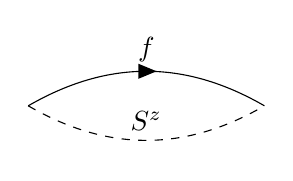
\begin{tikzpicture}
  %\feynmandiagram[large, horizontal=a to b] {
  %  a -- [fermion, edge label={abc\\$f$}, bend left] b,
  %  a -- [scalar, edge label=$S^z$, bend right] b};
  \begin{feynman}
    \vertex (a);
    \vertex[right=3cm of a] (b);
    \diagram*{
      (a) -- [fermion, edge label=$f$, bend left] (b),
      (a) -- [scalar, edge label=$S^z$, bend right] (b)
    };
  \end{feynman}
\end{tikzpicture}
\end{document}

